% Fundamentals of Microcontrollers Laboratory Manual
% 
% Manual to accompany the class lab
%
% Seth McNeill
% Started 2022 August 25

\documentclass[12pt,oneside]{book}
\usepackage[T1]{fontenc}  % to make underscores copy correctly
\usepackage{datetime}  % for automated current date on the document
\setcounter{secnumdepth}{3}  % to make subsubsections numbered
\usepackage{amsmath}  % for aligned equations and such
\usepackage[table]{xcolor}  % to color text
\usepackage[pdftex]{graphicx} % for includegraphics?
\usepackage{siunitx}  % for aligning tables by decimal point
\usepackage{pdfpages}  % to include PDF files in the document
\usepackage{listings}  % for code listings

% For creating nice addition figures
% based on https://tex.stackexchange.com/a/96764
\usepackage{cancel}
\usepackage{physics}  % for derivative symbols
\usepackage{tikz}
\usepackage{pdflscape}  % to make landscape pages that are turned in the pdf file
\usetikzlibrary{matrix, shapes, arrows.meta, positioning, angles, quotes}
\newcommand{\addend}{\text{\textsl{\color{gray}{Addend}}}}
\newcommand{\augend}{\text{\textsl{\color{gray}{Augend}}}}
\newcommand{\sumOut}{\text{\textsl{\color{gray}{Sum}}}}
% end addition figure requirements
\usepackage{hyperref}  % for URL hyperlinks

\hypersetup{
colorlinks,
citecolor=black,
filecolor=black,
linkcolor=blue,
urlcolor=blue
}

% setup listings for C++ and desired results
\lstset{ %
  backgroundcolor=\color{white},   % choose the background color; you must add \usepackage{color} or \usepackage{xcolor}
  basicstyle=\fontfamily{pcr}\selectfont,        % the size of the fonts that are   basicstyle=\fontfamily{psc}\selectfont,        % the size of the fonts that are used for the code
  breakatwhitespace=false,         % sets if automatic breaks should only happen at whitespace
  breaklines=true,                 % sets automatic line breaking
  captionpos=b,                    % sets the caption-position to bottom
%  commentstyle=\color{green},    % comment style
  escapeinside={\%*}{*)},          % if you want to add LaTeX within your code
  keepspaces=true,                 % keeps spaces in text, useful for keeping indentation of code (possibly needs columns=flexible)
  keywordstyle=\color{blue},       % keyword style
  language=C++,                 % the language of the code
  numbers=none,                    % where to put the line-numbers; possible values are (none, left, right)
  rulecolor=\color{black},         % if not set, the frame-color may be changed on line-breaks within not-black text (e.g. comments (green here))
  showspaces=false,                % show spaces everywhere adding particular underscores; it overrides 'showstringspaces'
  showstringspaces=false,          % underline spaces within strings only
  showtabs=false,                  % show tabs within strings adding particular underscores
  stringstyle=\color{black},     % string literal style
  tabsize=2,                       % sets default tabsize to 2 spaces
  title=\lstname                   % show the filename of files included with \lstinputlisting; also try caption instead of title
}


% for automated current date on the document
\newdateformat{myDate}{\THEYEAR{ }\monthname[\THEMONTH] \twodigit{\THEDAY}}

% Referencing commands 
\newcommand{\chaplabel}[1]{\label{chap:#1}}
\newcommand{\chapref}[1]{Chapter~\ref{chap:#1}}
\newcommand{\seclabel}[1]{\label{sec:#1}}
\newcommand{\secref}[1]{Section~\ref{sec:#1}}

\title{Fundamentals of Applied Microcontrollers Laboratory Manual}
\author{Seth McNeill}
\date{Edition Spring 2025 (v0.8) \\ \myDate\today}

\begin{document}
	\maketitle

	\tableofcontents
  \setcounter{chapter}{-1}
	% include chapters here
	\chapter{Introduction}
\chaplabel{intro}

This book is the accompanying lab manual to a class introducing microcontrollers
to upper division, non-electrical engineering undergraduate students who 
have taken some C programming.

If you find this useful, please let me know. If you find any errors, areas
that need improvement, or have any improvements to add please let me know.

The class textbook/manual is 
\href{https://github.com/semcneil/Fundamentals-of-Microcontrollers-Laboratories}{here}.

\section{License}
This code is released under a Creative Commons Attribution license.
The full text of the license is available at the following link.

\href{https://creativecommons.org/licenses/by/4.0/}{https://creativecommons.org/licenses/by/4.0/}

Users of this code should attribute the work to this
project by displaying a notice stating their product contains code
and/or text from the Fundamentals of Microcontrollers Project and/or linking to\\
https://github.com/semcneil/Fundamentals-of-Microcontrollers-Laboratories.
    \chapter{Arduino Startup}
\chaplabel{arduino}

<<<<<<< Updated upstream
section{Installing the IDE}
These directions assume that you are using the lab computers and One Drive.
=======
\section{Installing the IDE}
We want to try installing the IDE at least two different ways. First, on the lab computer, then on your personal
computers if you have them. Both lab partners should try installing the software on the lab computer, each with 
their own login.

\subsection{Lab Computer}
This method may also work on your personal computers.
\begin{enumerate}
    \item On the search bar, type in Microsoft Store.
    \item Click on Microsoft Store
    \item In the store search, type arduino
    \item Arduino IDE App should appear, click on it
    \item Click on Get
    \item You do not need to sign into Microsoft to make this install work even if prompted
    \item Once it has installed, run the Arduino IDE app. 
	\item It should load up with a window that looks like Figure \ref{fig:emptysketch}.
	\item Try rebooting the computer, logging in and seeing if the Arduino app is still present.
\end{enumerate}

\begin{figure}[!htb]
	\centering
	\includegraphics[scale=1.0]{arduinoStart/emptysketch.PNG}
	\caption{This is what the Arduino IDE should load up to.}
	\label{fig:emptysketch}
\end{figure} 

\subsection{Personal Computer}
>>>>>>> Stashed changes
\begin{enumerate}
	\item Go to software download page: \href{https://www.arduino.cc/en/software}{https://www.arduino.cc/en/software}
	\item Download the Windows ZIP file (not the first link or the app)
	\item Open the zip file and copy the folder inside (arduino-1.8.19 as of this writing) into your One Drive folder. This may take a while. If you are on your own computer, you can use any of the programs.
	\item Once that transfer finishes, go into the folder and run arduino.exe. Windows will try to save you, but if you click More Info you can click Run Anyway.
	\item Windows Defender Firewall will also complain. Uncheck the box that is checked and/or click Cancel.
	\item It should load up with a window that looks like Figure \ref{fig:emptysketch}.
	\item In order to get it to connect correctly to your board, you need to install the Arduino Nano Connect RP2040 board.
	\begin{enumerate}
		\item Navigate to Tools$\rightarrow$Board: ``Arduino Uno" (or similar)$\rightarrow$Boards Manager
		\item It should load as shown in Figure \ref{fig:boardsManager}.
		\item In the search bar, type ``arduino nano connect" (without the quotes)
		\item The first item should be Arduino Mbed OS Nano Boards and should list the Arduino Nano RP2040 Connect.
		\item Move your cursor over it and it should show an Install button. Click it to install the board library.
		\item Wait for it to finish.
		\item While you are waiting, plug your Nano Connect into your computer and let it install it.
		\item As it finished, I received a User Account Control warning asking if I wanted to let dpinst-amd64.exe make changes to my device. I said yes.
		\item Next it asked me if I wanted to install Arduino Universal Serial Bus devices. Again, click to Install.
		\item It popped up again and I clicked Install again. Now it should say that the Arduino Mbed OS Nano Boards has been installed.
		\item Close the Boards Manager.
	\end{enumerate}
	\item Now go to Files$\rightarrow$Examples$\rightarrow$01.Basics$\rightarrow$Blink.
	\item This will open another window with the Blink program.
	\item Go to Tools$\rightarrow$Board$\rightarrow$Arduino Mbed OS Nano Boards and select the Arduino Nano RP2040 Connect
	\item Go to Tools$\rightarrow$Port and select the COM that isn't COM1 (mine showed up as COM5)
	\item Click the right arrow under the word edit in the menu to Uplaod the sketch to the Arduino board.
	\item It should say ``Compiling sketch..." in the lower left and show a progress bar on the lower right.
	\item Then it should switch to Uploading... and finally Done Uploading.
	\item An orange light near the USB port on your board should be blinking.
	\item Congratulations! You have programmed your board!
	\item Now look in the program for the two delay statements. Try changing the values inside the parentheses and re-uploading it. Does the blinking change?
	\item In order to save files and have it portable, you need to change the directory where the Arduino IDE stores it's sketchbooks
	\begin{enumerate}
		\item Go to File$\rightarrow$Preferences
		\item Change the Sketchbook location to your OneDrive and a folder named arduino (lowercase is good)
		\item My OneDrive was in \\C:\textbackslash Users\textbackslash mcneils2\textbackslash OneDrive - Embry-Riddle 
		Aeronautical University\textbackslash arduino
	\end{enumerate}
	\item Now try saving the blink sketch with your changed values.
	\item Demonstrate your working blink and it's storage location to your instructor/TA
	\item Here are some other Examples to test:
	\begin{enumerate}
		\item Basics $\rightarrow$ fade: change the variable led to be LED\_BUILTIN, watch the red/orange LED pulse
		\item Analog $\rightarrow$ AnalogInOutSerial: change analogInPin to A1 and analogOutPin to LED\_BUILTIN. Turn 
				the potentiometer (R6) with a screwdriver and watch the LED change accordingly. If you press the magnifying
				glass button in the top right the actual values will scroll by. You may need to set the baud rate to 9600.
		\item Digital $\rightarrow$ DigitalInputPullup: Change the first pinMode call to use 9 instead of 2. The same for 
				the digitalRead command (2$\rightarrow$9). Press the left button and see the LED blink. The right button is 
				pin 10. Note that this program isn't written as well as the others since you have to change a number in two
				places. Could you rewrite it better?
	\end{enumerate}
    \item Finally, create a sketch called \lstinline$getIDs$ using the code at \\ 
        \href{https://github.com/semcneil/CEC325Examples/blob/main/getIDs/getIDs.ino}{https://github.com/semcneil/CEC325Examples/blob/main/getIDs/getIDs.ino}
    \item Run \lstinline$getIDs$ and submit the results in the end of lab Canvas quiz.
\end{enumerate}

\begin{figure}[!htb]
	\centering
	\includegraphics[scale=1.0]{arduinoStart/emptysketch.PNG}
	\caption{This is what the Arduino IDE should load up to.}
	\label{fig:emptysketch}
\end{figure} 

\begin{figure}[!htb]
	\centering
	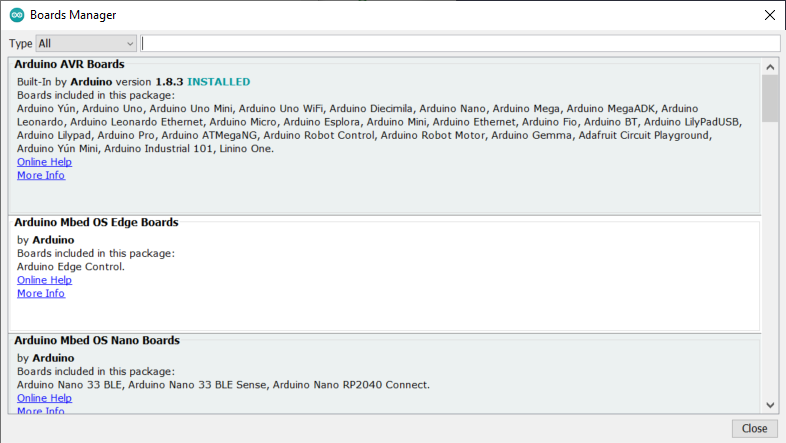
\includegraphics[scale=0.9]{arduinoStart/BoardsManager.PNG}
	\caption{This what the Boards Manager loads up to.}
	\label{fig:boardsManager}
\end{figure} 

\section{Turn In}
\begin{enumerate}
    \item Make sure that the TA or instructor has signed off on your modified blink sketch.
    \item Fill out the end of lab quiz prior to leaving. Note that it includes asking you 
            for the output of the \lstinline$getIDs$ sketch. 
\end{enumerate}

    \chapter{Multiplexer, LED Display, Binary, HEX}
\chaplabel{muxled}

\section{Purpose}
The goal of this lab is to use binary and hexadecimal numbers in an applied setting. This is 
achieved by having you (the student) use the Arduino Nano Connect RP2040 to setup the 
PCA9535 I$^2$C Input/Output (IO) port chip to drive a 4-digit LED display.

\section{Resources}\label{sec:resources}
\begin{enumerate}
    \item \href{https://www.nxp.com/products/interfaces/ic-spi-i3c-interface-devices/general-purpose-i-o-gpio/16-bit-ic-bus-and-smbus-low-power-i-o-port-with-interrupt:PCA9535_PCA9535C}{PCA9535 datasheet}
    \item \href{https://datasheet.lcsc.com/lcsc/1810191633_SUNLIGHT-SLR0394FG3C5BD-3-5_C225905.pdf}{LED display datasheet}
 %   \item \href{https://github.com/semcneil/PCA95x5}{PCA9535 library} (McNeill version)
    \item PCB Schematic and Layout - see 
            \href{https://github.com/semcneil/Fundamentals-of-Microcontrollers-Manual}{class manual} 
            in the Arduino Startup $\rightarrow$ Schematics and PCB section
\end{enumerate}

\section{Procedure}
\subsection{Add the PCA95x5 library}
In Sketch $\rightarrow$ Include Library $\rightarrow$ Manage Libraries search for 
PCA9535 and install the latest version of the one by hideakitai.
% Normally libraries can be added by using the Arduino IDE library manager. However, this 
% library hasn't been included in it yet, so you will install it by hand. This is an 
% important skill to know since not all the software you will need to use is in the 
% normal library system.

% \begin{enumerate}
%     \item Open the Arduino IDE 
%     \item Open preferences
%     \item Note the Sketchbook location 
%     \item Go to the website for the PCA9535 library (see \ref{sec:resources} Resources section)
%     \item Click the green Code button and then Download ZIP
%     \item Save the zip file to your Downloads folder or somewhere else you can find it again
%     \item In the Arduino IDE select Sketch $\rightarrow$ Include Library $\rightarrow$ Add .ZIP Library
%     \item Select the zip file you downloaded earlier
%     \item Wait for the IDE to say ``Library added to your libraries"
%     \item Check that the library is indeed installed one of two ways:
%     \begin{enumerate}
%         \item Go to Sketch $\rightarrow$ Include Libraries and look for PCA95x5
%         \item Go to File $\rightarrow$ Examples and look for the PCA95x5 examples
%     \end{enumerate}
%     \item The PCA95x5 library is now added successfully.
% \end{enumerate}

\subsection{Turn on some LEDs}
An example script is shown in Listing \ref{lst:leddispstart}. Use this as a starting point for your
code. Be sure to change the header information to include all lab partner names and the correct 
date. This script displays an 8. in the first digit and zeros in the rest. Note the clearing
lines to make it so that there is not ghosting of numbers to the right of where they are displayed. 
Remember that we are using the PCA9535 chip which requires the PCA95x5 library. When using a library 
the following steps must be followed or else the microcontroller will probably crash or at least 
the part you are trying to use will not work. Note the steps in Listing \ref{lst:leddispstart}.

\begin{enumerate}
    \item Include the library: \lstinline|#include <PCA95x5.h>|
    \item Create an object: \lstinline|PCA9535 LEDmux;|
    \item Initialize the object: usually a \lstinline|.begin()| method (PCA9535 requires more)
    \item Use the object: \lstinline|LEDmux.write(0xFF0E);|
\end{enumerate}

Now to begin showing some numbers on the 7-segment display.

\begin{enumerate}
    \item Run the script in Listing \ref{lst:leddispstart} to make sure it runs. Beware of copying
            multiple lines from a PDF to the Arduino IDE since it often adds in unwanted characters. 
            Also, underscores (\_) and some other symbols sometimes fail to transfer correctly. The 
            sketch is also available for download from the class Canvas site.
    \item Change the script so that it displays four consecutive numbers such as 1234. You can use
            any 4 consecutive, single digit numbers.
    \item Demonstrate your sketch working to a TA or instructor.
\end{enumerate}

\begin{lstlisting}[language=C++, caption={This listing is a starting point for driving the LED display. 
    This sketch may also be available on Canvas. Beware of copying out of PDFs since some characters
     (underscore for instance) come through garbled.},label={lst:leddispstart}]
    /* 20220907LEDsClass1.ino
    *  
    * Demo of LED display in class.
    * 
    * Seth McNeill
    * 2022 September 07
    */
   
   #include <PCA95x5.h>  // include library
   
   PCA9535 LEDmux;  // create instance (object) of library
   
   void setup() {
     Serial.begin(115200);
     delay(3000);
     Serial.println("Starting...");
   
     // initialize object
     Wire.begin();  // this must be done before LEDmux.attach
     LEDmux.attach(Wire, 0x21);  // 0x21 is the I2C address for the PCA9535 attached to the LEDs
     LEDmux.polarity(PCA95x5::Polarity::ORIGINAL_ALL);
     uint16_t mux_direction = 0x0010;  // mostly outputs (0), setting to 1 designates input
     LEDmux.direction(mux_direction);
   
     Serial.println("Everything setup");
   }
   
   
   void loop() {
     int delayTime = 0;
     // use object
     LEDmux.write(0x000F);  // required to remove ghosting on other digits
     LEDmux.write(0xFF0E);
     delay(delayTime); 
     LEDmux.write(0x000F);  // required to remove ghosting on other digits
     LEDmux.write(0x3F0D);
     delay(delayTime); 
     LEDmux.write(0x000F);  // required to remove ghosting on other digits
     LEDmux.write(0x3F0B);
     delay(delayTime); 
     LEDmux.write(0x000F);  // required to remove ghosting on other digits
     LEDmux.write(0x3F07);
     delay(delayTime); 
   }
\end{lstlisting}
Note the anti-ghosting lines in Listing \ref{lst:leddispstart}. This is because the two
bytes on the PCA9535 do not change simultaneously. One will change before the other 
giving a slight showing of the previous number before showing the new number. The fix 
is to turn off all four segments before writing the new number.
    
\subsection{Count}
Make a new sketch, based off your first sketch (meaning copy and paste it into the new sketch).
This new sketch should count up from 0 to 9 (or 0000 to 0009) incrementing once per second. Demonstrate
this counting to a TA/instructor and get it signed off.

\subsection{Extra credit: 2 pts}
Have your counting system count in increments of 1 using more than one digit (i.e. 
count from 00 to 99 if two digits). You must do the full count to 99, 999, or 9999,
not just count to 10. It should reset (overflow) back to zero and keep counting 
when it reaches the maximum. 
\subsection{Extra Credit Hints}
\begin{enumerate}
    \item Use the \lstinline|millis()| function to update count every second. The 
            following \lstinline|if| statement shows an example of how to do this: \\
            \lstinline|if(millis() - lastUpdate > updateInterval)|
    \item I used an array for the segments required for each number something like \\
            \lstinline|nums[] = {0xAB,0x1C,...}|  // values not correct
    \item I also used an array to specify which digit is showing, something like \\
            \lstinline|digs[] = {0x12, 0x0E,...}| // values not correct
    \item These can be combined since \lstinline|nums[ii]| is the upper byte and 
            \lstinline|digs[jj]| is the lower byte of the number that needs to be 
            written to the PCA9535. \lstinline|nums[ii]| needs to be shifted to be 
            the upper byte using the \lstinline|<<| operator. For example: \\
            \lstinline@(nums[ii] << 8) | digs[jj]@ 
\end{enumerate}

\section{Turn In}
Turn in the following:
\begin{enumerate}
    \item Make sure that you have been signed off for both consecutive numbers and counting.
    \item A PDF of your first sketch that displays 4 consecutive numbers.
    \item A PDF of your second sketch that counts.
    \item .ino versions of both sketches.
    \item Fill out the end of lab quiz prior to leaving. Note that it includes asking you 
            for the output of the \lstinline$getIDs$ sketch. 
\end{enumerate}
    \chapter{Buttons and Serial (UART)}
\chaplabel{buttonserial}

\section{Purpose}
The goal of this lab is to gain a better understanding of the serial interface between
the board and the computer, get the buttons all working, and add a few other fun interfaces. 

Note that the most time consuming part of this lab in 2022 was getting the non-SW1 switches
working.

\subsection{Serial Library}
\subsubsection{Initialization}
So far we have used the Serial library without much explanation of how to use it best.
In the sketches we have used we just have used the two lines shown in 
Listing~\ref{lst:simpleserialstart} to start Serial.

\begin{lstlisting}[language=C++, caption={If serial is required for a sketch this method of 
    starting Serial blocks until a serial monitor is started.},label={lst:simpleserialstart}]
    Serial.begin(115200);
    while(!Serial);
\end{lstlisting}

However, if a serial connection to the computer is not required, the code in 
Listing~\ref{lst:simpleserialstart} prevents the rest of the sketch from executing. The Serial
library does take some time to start so a simple solution is to just delay for a few seconds
after calling \lstinline$Serial.begin()$ as shown in Listing~\ref{lst:serialstartdelay}.

\begin{lstlisting}[language=C++, caption={If serial is not required for a sketch this method of 
    starting Serial waits a bit in hopes it connects.},label={lst:serialstartdelay}]
    Serial.begin(115200);
    delay(3000);
\end{lstlisting}

If you want to have the program quit waiting as soon as the Serial connects but not delay forever
like in Listing~\ref{lst:simpleserialstart}, you can keep checking for a serial connection a fixed
number of times as shown in Listing~\ref{lst:serialstartdelay}.

\begin{lstlisting}[language=C++, caption={This snippet tries connecting to Serial a fixed 
    number of times so that it will delay less than Listing~\ref{lst:serialstartdelay} if 
    a serial connection exists.},label={lst:serialstartcount}]
    const int maxNoSerial = 300;
    int noSerialCount = 0;
    while(!Serial && noSerialCount < maxNoSerial) {
      delay(10);
      noSerialCount++;
    }
\end{lstlisting}

\subsubsection{print vs println}
If you want to print a string with an endline, use \lstinline$Serial.println()$. This is 
handy for statements like \lstinline$Serial.println("Starting...")$. However, if you 
want to print out the value of variables you often don't want newline at the end of
the print. For this you use \lstinline$Serial.print()$. Some examples are shown in 
Listing~\ref{lst:serialprintprintln}.
\begin{lstlisting}[language=C++, caption={This snippet shows using print and println},label={lst:serialprintprintln}]
    Serial.print("Number of Names: ");
    Serial.println(nNames);
    ...
    Serial.print(F("You're connected to the network, IP = "));
    Serial.println(WiFi.localIP());    
\end{lstlisting}

\subsubsection{Reading data from the Serial}
The serial connection goes both ways. Information can be sent from the computer to 
your board. Listing~\ref{lst:serialreceiveexample} is an example of using input from 
the serial port. The call to \lstinline$Serial.available()$ tells the sketch whether
or not any characters have been received by the serial port. If characters have been
received by the serial port, \lstinline$Serial.read()$ reads them in one character at 
a time. The \lstinline$switch$ function allows different responses depending on what 
character is received. 

Note the layout of the sketch. It is important to define the pins for accessories so 
that they can be used later. 

\begin{lstlisting}[language=C++, caption={This sketch shows controlling parts of the 
    board using input from the serial port. Remember, don't copy and paste from a PDF
    since that process garbles some of the characters.},label={lst:serialreceiveexample}]
    /*  CEC325-SerialRcv.ino
    *  
    *  Demonstrates receiving and reacting to serial input.
    *  Uses the ERAU CEC325 board v0.3 which has an 
    *  Arduino Nano RP2040 Connect on board.
    *  
    *  Seth McNeill
    *  2022 February 09
    *  2022 September 20 modified for v0.5 board
    *  
    *  This code in the public domain.
    */
   
   #include <WiFiNINA.h>  // for RGB LED
   
   // pin definitions:
   #define RIGHT_BUTTON_PIN  A0 
   #define BUZZ_PIN          2 // buzzer
   
   
   void setup() {
     // initialize serial:
     Serial.begin(115200);
     while(!Serial) delay(100); // Require serial
     Serial.println("Starting...");
     
     // make the pins outputs:
     pinMode(LEDR, OUTPUT);  // WiFiNINA RGB LED red
     pinMode(LEDG, OUTPUT);  // WiFiNINA RGB LED green
     pinMode(LEDB, OUTPUT);  // WiFiNINA RGB LED blue
     pinMode(RIGHT_BUTTON_PIN, INPUT);  
     pinMode(LED_BUILTIN, OUTPUT);
     pinMode(BUZZ_PIN, OUTPUT);  // buzzer pin is output
   }
   
   void loop() {
     while(Serial.available() > 0) {  
       // characters have been received
       char inChar = Serial.read();
       switch(inChar) {
         case 'a': digitalWrite(LED_BUILTIN,HIGH); break;
         case 'A': digitalWrite(LED_BUILTIN,LOW); break;
         case 'b': digitalWrite(LEDB, HIGH); break;
         case 'r': digitalWrite(LEDR, HIGH); break;
         case 'g': digitalWrite(LEDG, HIGH); break;
         case '+': add(); break;
         case 'o': ledsOff(); break;
         case 'z': tone(BUZZ_PIN, 1000, 100); break;
         case '\n': break;
         default: Serial.print("Unknown character: "); Serial.println(inChar);
       }
     }
   }
   
   // turns off all 4 LEDs
   void ledsOff() {
     digitalWrite(LED_BUILTIN,LOW);
     digitalWrite(LEDR,LOW);
     digitalWrite(LEDG,LOW);
     digitalWrite(LEDB,LOW);
   }
   
   // Adds characters received subsequent to +
   void add() {
     Serial.println("Adding single digit numbers");
     int a = Serial.read() - 48; // subtract off value of ASCII 0
     int b = Serial.read() - 48; // subtract off value of ASCII 0
     Serial.print(a);
     Serial.print('+');
     Serial.print(b);
     Serial.print('=');
     Serial.println(a+b);
   }   
\end{lstlisting}


\subsection{Buttons}
\subsubsection{I/O Setup}
To use general I/O pins on a processor in Arduino the pin has to be defined as an 
input or an output. This is done in the \lstinline$setup()$ function using the 
\lstinline$pinMode()$ function. It has the form of 
\lstinline$pinMode(pinNumber, direction)$. The pinNumber is typically the number 
defined in the Arduino specifications as D1 or A0. If it is a D1 type number, then
just pass the number to pinMode. If it is an A0 type number, you have to specify 
both the letter and the number. So for the righthand button (SW1) on the v0.5 board 
that is attached to the A0 pin you would use \lstinline$pinMode(A0, INPUT)$ since
it is an input. The buzzer is attached to pin D2 so we would set it up as 
\lstinline$pinMode(2, OUTPUT)$ since it is an output. 

\subsubsection{Reading and Writing Pins}
Once the pinMode has been setup, you can read the value from an input using the 
\lstinline@digitalRead(pinNum)@ function which takes a pin number as an argument
and returns a 1 or 0 (LOW or HIGH) depending on the read value.

To write a value to an output pin, use the \lstinline@digitalWrite(pinNum, value)@ 
function. It also takes a pin number as an input along with whether you want the 
output LOW or HIGH. 

Since you will be using the pin number in multiple places, it is best to define it 
with a name at the top of the program so that you can change it at all places in 
your program by changing it once.

Examples of writing pins after setting their mode can be seen in 
Listing~\ref{lst:serialreceiveexample}.

\subsubsection{Other buttons}
The v0.5 board has 4 buttons. SW1 is attached to A0 and can be read directly using
\lstinline@digitalRead@. The other three buttons (SW2, FRONT\_SW, and BACK\_SW) are 
connected to the PCA9535 I2C to GPIO chip with an address of 0x20 and have to be 
accessed using the PCA95x5 library. 

%Remember to install the McNeill version of the PCA95x5 library from a Github zip 
%file, not the library from the standard Arduino library manager.
Remember to install the PCA95x5 library as follows:
In Sketch $\rightarrow$ Include Library $\rightarrow$ Manage Libraries search for 
PCA9535 and install the latest version of the one by hideakitai.

\begin{enumerate}
    \item Include the PCA95x5 library
    \item Create a global variable of type PCA9535 named something like \lstinline@muxU31@ 
            (for the chip listed as U31 on the schematic)
    \item Initialize the variable/object inside the \lstinline|setup()| function:
    \begin{enumerate}
        \item Start the wire library: \lstinline@Wire.begin()@
        \item Attach to the mux using the attach method and correct address: 
                \lstinline@muxU31.attach(Wire, 0x20)@
        \item Set the polarity: \lstinline@muxU31.polarity(PCA95x5::Polarity::ORIGINAL_ALL)@ 
        \item Set the direction: \lstinline@muxU31.direction(0x????)@ remembering that a 1 is 
                an input and a 0 is an output. Set non-connected pins as outputs. Change the 
                question marks appropriately by looking at the schematics in the Class Manual 
                linked to in the \nameref{sec:buttonserialresources} Section.
    \end{enumerate}
    \item Once the object is properly setup, read values with the \lstinline@read()@ 
            method. This returns a 16-bit number representing the 16 inputs on the chip.
    \item A quick way to check if a bit is high is to bitwise AND (\&) it with a number 
            where only the bit of interest is 1: \lstinline@mux31.read() & 0x0004@ reads 
            the third input.
\end{enumerate}

Note that switches SW1 and SW2 are are HIGH when not pressed and LOW 
when pressed while FRONT\_SW and BACK\_SW are LOW when not pressed and HIGH when pressed.

\begin{lstlisting}[language=C++, caption={The buttons attached to the PCA9535 can be accessed 
    as shown in this code snippet.},label={lst:muxButtons}]
    uint16_t muxVal = muxU31.read();
    if(muxVal & 0x0001) {
        // Do something with left button
    }
    if(muxVal & 0x0002) {
        // Do something with another button
    }
\end{lstlisting}



\subsection{Making Noise (buzzer)}
The board for lab has a buzzer attached to pin D2. Arduino has a handy function called 
\lstinline@tone(pin, frequency, duration)@. This is an easy way to make your board beep.
The duration is in milliseconds and the function blocks until the duration expires. Note 
that there is another version of the function with the form 
\lstinline@tone(pin, frequency)@ that does not specify a duration. This is a non-blocking
way to make tones. It will continue to make the tone until a call to \lstinline@noTone(pinNum)@
is called. 

\textbf{NOTE:} If the tone function is all that is in a loop, it needs a short delay (10~ms will do)
after it to keep the Nano Connect RP2040 from crashing.

\subsection{NeoPixels}
The board has 18 multicolor LEDs around its periphery. These are called NeoPixels by the 
Adafruit company. They get called other things by other companies. They are all based on 
the WS2812 type chip. We will use the Adafruit NeoPixel library. Be sure to install it 
in the usual manner in the Library Manager. It requires the usual:
\begin{enumerate}
    \item \#include the library
    \item Initialize an object
    \item Setup the library
    \item Use the library
\end{enumerate}
A minimal sketch to do all these is shown in Listing~\ref{lst:neopixelsetup}

\begin{lstlisting}[language=C++, caption={This snippet shows how to setup and run the NeoPixels on the board.},label={lst:neopixelsetup}]
    /* NeoPixelSetup.ino
    * 
    * A minimum sketch to setup NeoPixels.
    * 
    * Seth McNeill
    * 2022 September 20
    */
   
   #include <Adafruit_NeoPixel.h> // NeoPixel library
   
   #define NEO_PIN           17  // WARNING! THIS IS GPIO NOT D NUMBER for NeoPixels
   #define NEO_COUNT         18  // number of NeoPixels
   
   // Declare our NeoPixel strip object:
   Adafruit_NeoPixel strip(NEO_COUNT, NEO_PIN, NEO_GRB + NEO_KHZ800);
   
   void setup() {
     Serial.begin(115200);
   
     // Setup NeoPixels
     strip.begin();
     strip.clear();  // Set all pixel values to zero
     strip.show();   // Write values to the pixels
   }
   
   void loop() {
     for(int ii = 0; ii < NEO_COUNT; ii++) {
       // set all the pixels to purple
       strip.setPixelColor(ii, strip.Color(255,0,255));
     }
     strip.show();
     delay(1000);
     // turn off all the LEDs
     strip.clear();
     strip.show();
     delay(1000);
   }   
\end{lstlisting}

\section{Resources}\label{sec:buttonserialresources}
\begin{enumerate}
    \item \href{https://www.arduino.cc/reference/en/language/functions/communication/serial/}{Serial Library}
    \item \href{https://www.arduino.cc/reference/en/language/functions/digital-io/digitalread/}{digitalRead}
    \item \href{https://www.arduino.cc/reference/en/language/functions/advanced-io/tone/}{tone}
    \item \href{https://www.arduino.cc/reference/en/language/functions/advanced-io/notone/}{notone}
%    \item \href{https://github.com/adafruit/Adafruit_SHT31}{Adafruit's SHT31 library}
%    \item \href{https://github.com/RobTillaart/SHT31}{Rob Tillaart's SHT31 library}
    \item \href{https://www.arduino.cc/reference/en/libraries/adafruit-neopixel/}{Adafruit NeoPixel Library}
    \item \href{https://www.nxp.com/docs/en/data-sheet/PCA9535_PCA9535C.pdf}{PCA9535 datasheet}
    \item \href{https://github.com/semcneil/PCA95x5}{PCA9535 library} (McNeill version)
    \item PCB Schematic and Layout - see 
            \href{https://github.com/semcneil/Fundamentals-of-Microcontrollers-Manual}{class manual} 
            in the Arduino Startup $\rightarrow$ Schematics and PCB section
\end{enumerate}

\section{Procedure}
Write a sketch with the following functionality:
\begin{enumerate}
    \item Reacts to all 4 buttons on the board in some way such as sound, light, or Serial. 
            THIS IS THE HARDEST PART. START HERE.
    \item Reads in values from the serial port and does something in response.
    \item Writes information to the serial port in response to some stimulus/stimuli.
    \item Creates a tone in response to some stimulus.
    \item Make the NeoPixels do something.
\end{enumerate}

\section{Debugging}
Here are some pointers to help if your program gives errors:
\begin{enumerate}
    \item Missing \lstinline|Wire.h|: Make sure you are including the PCA95x5 library
    \item Upload just gives a series of dots and says upload failed.
    \begin{enumerate}
        \item Check to make sure the correct COM port is selected in Tools menu
        \item Try pressing the reset button twice to put the RP2040 in upload mode 
        \item If nothing works, bring your board to the professor/TA to have a hard reset performed
    \end{enumerate}
    \item ``Out of scope'' errors. Count and match curly brackets (\{\}) to make sure all
                your code is inside \lstinline|setup()| or \lstinline|loop()|. The only code
                that can be outside of a function is a variable declaration (e.g. \lstinline|int x|)
\end{enumerate}

\section{Turn In}
Turn in the following:
\begin{enumerate}
    \item Make sure that the TA/Instructor signs off on your sketch demonstration.
    \item A PDF of your sketch.
    \item .ino versions of your sketch.
    \item Fill out the end of lab quiz prior to leaving. Note that it includes asking you 
            for the output of the \lstinline$getIDs$ sketch. 
\end{enumerate}
    \chapter{Displays}
\chaplabel{displays}

\section{Purpose}
The goal of this lab is to learn to use the TFT display.

\section{Procedure}
\subsection{Main Requirements}
Write a sketch with the following functionality:
\begin{enumerate}
    \item Display a custom message for 3~seconds indicating the start of the program when
            your program starts 
    \item Choose a favorite character and have it move left 10~pixels for each press
            of the left button and right 10~pixels for each press of the right button.
    \begin{enumerate}
        \item Choose the Y value to be one that looks good to you
        \item If 10~pixels seems to not be a good value feel free to change it, just note
                that you changed the value
        \item This builds on last week's making all the buttons function
        \item Debounce the buttons so that each press only moves the character once
        \item Add logic so that the character doesn't go far off the edge of the screen
                on either side.
    \end{enumerate}
    \item Draw some (at least 3, but they don't all have to be different) of the 
            drawing primitives (line, circle, rectangle, etc.)
\end{enumerate}

\subsection{Extra Credit}
The following are extra credit options with increasing value:
\begin{enumerate}
    \item Make the front and back switches move your character up and down along 
            with the left and right from the Main Requirements. (1~point)
    \item Make an animation of some kind that lasts at least two seconds. (1~points)
    \item Make a game that uses the buttons and the screen (2~points)
\end{enumerate}

\section{Turn In}
Turn in the following:
\begin{enumerate}
    \item Make sure that the TA/Instructor signs off on your sketch demonstration.
    \item A PDF of your sketch.
    \item .ino versions of your sketch.
    \item Fill out the end of lab quiz prior to leaving. Note that it includes asking you 
            for the output of the \lstinline$getIDs$ sketch. 
\end{enumerate}

\section{Resources}\label{sec:displaysresources}
\begin{enumerate}
    \item \href{https://www.adafruit.com/product/4383}{Adafruit 1.14" 240x135 Color TFT Display + MicroSD Card Breakout - ST7789}
    \item \href{https://www.arduino.cc/reference/en/libraries/adafruit-st7735-and-st7789-library/}{Adafruit ST7789 library}
    \item \href{https://learn.adafruit.com/adafruit-gfx-graphics-library}{Adafruit GFX library}
    \item See the chapter in the \href{https://github.com/semcneil/Fundamentals-of-Microcontrollers-Manual}{class manual} about displays
    \item PCB Schematic and Layout - see 
            \href{https://github.com/semcneil/Fundamentals-of-Microcontrollers-Manual}{class manual} 
            in the Arduino Startup $\rightarrow$ Schematics and PCB section
\end{enumerate}


    \chapter{Environmental Sensing}
\chaplabel{envSensing}

\section{Purpose}
The goal of this lab is to learn to collect data with an ADC and other sensors.

\section{Procedure}
\subsection{Main Requirements}
Write a sketch with the following functionality:

Collect the following data and display it once every 5 seconds via serial and on the display with the 
appropriate labels and units if you can make them fit.
\begin{enumerate}
	\item The output from \lstinline@millis()@ (ms)
	\item Both light intensities as a number between 0 and 1023 (unitless)
	\item Potentiometer value as a voltage between 0 and 3.3~V
	\item Temperature in Fahrenheit from TEMP0 (U27 attached to input 0 of U37)
    \item Get SHT31 reporting temperature in F and humidity via Serial
    \item Add SHT31 data to display 
    \item Get compass (QMC5883L) reporting azimuth via Serial
    \item Add azimuth data to the display
    \item Get IMU (LSM6DSOX) reporting accelerations and gyroscope data via Serial 
    \item Add accelerometer and gyroscope data to display
    \item Get 1-Wire (DS18B20) sensor(s) reporting temperature(s) via Serial
    \item Display 1-Wire temperature(s) on display
\end{enumerate}

The light sensors, potentiometer, and temperature sensor are connected to ADS7142 
analog-to-digital (ADC) sensors. There is a library in the normal library adding 
method. Look for the library for the ADS7142 by Seth McNeill. After you install it,
there should now be examples under Anitracks ADS7142. Follow the read2Ch example 
combined with your previous work to complete this lab.

\subsection{Suggestions}
Use a \href{https://www.arduino.cc/reference/en/language/variables/data-types/stringobject/}{String} 
object to accumulate your display string and then call \lstinline@display.println(yourString)@ 
to display it. Note a few things:
\begin{enumerate}
	\item The String type starts with a capital S.
	\item You can add to the String object using \lstinline@+=@ or just \lstinline@+@, 
		but with only the plus operator, all arguments have to be of the same type. 
	\item The String object also allows you to limit the number of decimal places for \lstinline@float@ types.
            \lstinline@String(tF,1)@ displays tF to 1 decimal place.
\end{enumerate}
An example is shown in Listing \ref{lst:dispstr}.
\begin{lstlisting}[caption={This is an example of using a String 
		object to display text and float variables. The floats are 
		limited to 1 decimal place such that 7.123 would be displayed as 7.1.},
		label={lst:dispstr},language=C++]
	String dispStr;
	dispStr = "T(F): ";
	dispStr += String(tF,1);
	dispStr += "\n";
	// Control the display  
	tft.fillScreen(ST77XX_BLACK);  // clear display
	tft.setTextColor(ST77XX_YELLOW);  // set text color
	tft.setTextSize(1);  // Normal 1:1 pixel scale
	tft.setCursor(0,0);  // Start at top-left corner
	tft.println(dispStr);
\end{lstlisting}
However, if you want to have different portions of the text in different colors you will
need to call \lstinline@tft.setTextColor@ between each \lstinline@tft.println@.

\subsection{SHT31 Temperature and Humidity Sensor}
Use Adafruit's SHT31 library. Base your code on their example. Be sure 
to make sure that the heater is off. For this class, you do not need to 
turn on the heater.

Also, the SHT31 needs to be reset each time the program starts. It's 
reset pin is connected to a PCA9535. Don't forget to use the 
\href{https://github.com/semcneil/PCA95x5}{PCA95x5 library written by Seth McNeill}, 
not the one in the Arduino library manager. An example of how to do this
is shown in Listing \ref{lst:sht31reset}.

\begin{lstlisting}[caption={This listing shows how to reset the SHT31.},
label={lst:sht31reset},language=C++]
Wire.begin();
muxU31.attach(Wire, 0x20);
muxU31.polarity(PCA95x5::Polarity::ORIGINAL_ALL);
muxU31.direction(0x1CFF);  // 1 is input, see schematic to get upper and lower bytes
muxU31.write(PCA95x5::Port::P08, PCA95x5::Level::L);  // disable SHT31
delay(100);
muxU31.write(PCA95x5::Port::P08, PCA95x5::Level::H);  // enable SHT31
delay(100);

Serial.println("SHT31 test");
if (! sht31.begin(0x44)) {   // Set to 0x45 for alternate i2c addr
    Serial.println("Couldn't find SHT31");
    while (1) delay(1);
}
\end{lstlisting}

\subsection{QMC5883L Compass}
Use the library by MRPrograms for the QMC5883L compass. The azimuth example 
should provide what you need to make it go.

\subsection{LSM6DSOX IMU}
Install the Arduino library for the LSM6DSOX IMU. Your program will need 
to use a combination of the SimpleAccelerometer and SimpleGyroscope examples.
NOTE: This library returns acceleration in g's not $m/s^2$.

\subsection{1-Wire Sensors}
As mentioned in class, the only library I have found to work with the Nano Connect 
RP2040 is the \href{https://github.com/pstolarz/OneWireNg}{OneWireNg} library. 
Unfortunately, the library examples are very complex. There is a simpler solution by 
combining the examples from the OneWire library with the capabilities of the OneWireNg 
library. It has to be done carefully though. Here is how to do it:
\begin{enumerate}
    \item In the Arduino IDE install both the OneWire and OneWireNg libraries
    \item Open the OneWire example named \lstinline@DS18x20_Temperature@ 
    \item Make the first \lstinline|#include| in your file be:\\
            \lstinline@#include "OneWireNg_CurrentPlatform.h"@ 
    \item This example should now compile and run just fine 
\end{enumerate}

\subsubsection{NOTE}
This example reads the results from one (1) sensor per pass through the 
\lstinline@loop()@ function. For your program, you will want to collect 
all three sensors' data in a single pass through the \lstinline@loop()@ 
function. 

Start by just reading one DS1820 then after you have everything
else working, come back and add in the rest of the DS1820 sensors.

\section{Main Requirements}
Write a sketch with the following functionality:

Collect the following data and display it once every 5 seconds via serial and on 
the display with the appropriate labels and units if you can make them fit.
\begin{enumerate}
	\item The output from \lstinline@millis()@ (ms)
	\item Both light intensities as a number between 0 and 1023 (unitless)
	\item Potentiometer value as a voltage between 0 and 3.3~V
	\item Temperature in Fahrenheit from TEMP0 (U27 attached to input 0 of U37)
	\item The temperature in Fahrenheit and humidity from the SHT31 sensor
	\item The compass azimuth angle
	\item The 3-axis accelerometer and gyroscope data (6 data points)
 	\item The temperatures from at least one 1-Wire DS18B20 sensor (can take about
            seconds for acquisition for 3 sensors). Do this part last.
\end{enumerate}

\section{Turn In}
Turn in the following:
\begin{enumerate}
    \item Have either the TA or the instructor sign-off on your lab
    \item A PDF of your sketch.
    \item .ino versions of your sketch.
    \item Fill out the end of lab quiz prior to leaving. Note that it includes asking you 
            for the output of the \lstinline$getIDs$ sketch. 
\end{enumerate}

\section{Resources}\label{sec:datacollectionsresources}
\begin{enumerate}
    \item \href{https://www.adafruit.com/product/4383}{Adafruit 1.14" 240x135 Color TFT Display + MicroSD Card Breakout - ST7789}
    \item \href{https://www.arduino.cc/reference/en/libraries/adafruit-st7735-and-st7789-library/}{Adafruit ST7789 library}
    \item \href{https://learn.adafruit.com/adafruit-gfx-graphics-library}{Adafruit GFX library}
    \item The \href{https://sensirion.com/products/catalog/SHT31-DIS-B/}{SHT31 temperature and humidity sensor datasheet}
    \item The \href{https://www.filipeflop.com/img/files/download/Datasheet-QMC5883L-1.0%20.pdf}{QMC5883L compass datasheet}
    \item The \href{https://www.st.com/resource/en/datasheet/lsm6dsox.pdf}{LSM6DSOX IMU datasheet}    \item See the chapter in the \href{https://github.com/semcneil/Fundamentals-of-Microcontrollers-Manual}{class manual} about displays
    \item The \href{https://cdn-shop.adafruit.com/datasheets/DS18B20.pdf}{DS18B20 temperature sensor datasheet}
    \item PCB Schematic and Layout - see 
            \href{https://github.com/semcneil/Fundamentals-of-Microcontrollers-Manual}{class manual} 
            in the Arduino Startup $\rightarrow$ Schematics and PCB section
\end{enumerate}


    %\chapter{More Sensors}
\chaplabel{moreSensors}

\section{Purpose}
The goal of this lab is to learn to collect data with more sensors.

\section{Procedure}
It is best to follow this outline to finish this lab most efficiently.
\begin{enumerate}
    \item Get 1-Wire (DS18B20) sensors reporting temperatures via Serial
    \item Display 1-Wire temperatures on display
    \item Get SHT31 reporting temperature and humidity via Serial
    \item Add SHT31 data to display 
    \item Get compass (QMC5883L) reporting azimuth via Serial
    \item Add azimuth data to the display
    \item Get IMU (LSM6DSOX) reporting accelerations and gyroscope data via Serial 
    \item Add accelerometer and gyroscope data to display
\end{enumerate}

\subsection{1-Wire Sensors}
As mentioned in class, the only library I have found to work with the Nano Connect 
RP2040 is the \href{https://github.com/pstolarz/OneWireNg}{OneWireNg} library. 
Unfortunately, the library examples are very complex. There is a simpler solution by 
combining the examples from the OneWire library with the capabilities of the OneWireNg 
library. It has to be done carefully though. Here is how to do it:
\begin{enumerate}
    \item In the Arduino IDE install both the OneWire and OneWireNg libraries
    \item Open the OneWire example named \lstinline@DS18x20_Temperature@ 
    \item Add this line above the \lstinline@#include <OneWire.h>@ line:\\
            \lstinline@#include "OneWireNg_CurrentPlatform.h"@ 
    \item This example should now compile and run just fine 
\end{enumerate}

\subsubsection{NOTE}
This example reads the results from one (1) sensor per pass through the 
\lstinline@loop()@ function. For your program, you will want to collect 
all three sensors' data in a single pass through the \lstinline@loop()@ 
function.

\subsection{SHT31 Temperature and Humidity Sensor}
Use Adafruit's SHT31 library. Base your code on their example. Be sure 
to make sure that the heater is off. For this class, you do not need to 
turn on the heater.

Also, the SHT31 needs to be reset each time the program starts. It's 
reset pin is connected to a PCA9535. Don't forget to use the 
\href{https://github.com/semcneil/PCA95x5}{PCA95x5 library written by Seth McNeill}, 
not the one in the Arduino library manager. An example of how to do this
is shown in Listing \ref{lst:sht31reset}.

\begin{lstlisting}[caption={This listing shows how to reset the SHT31.},
label={lst:sht31reset},language=C++]
Wire.begin();
muxU31.attach(Wire, 0x20);
muxU31.polarity(PCA95x5::Polarity::ORIGINAL_ALL);
muxU31.direction(0x1CFF);  // 1 is input, see schematic to get upper and lower bytes
muxU31.write(PCA95x5::Port::P08, PCA95x5::Level::L);  // disable SHT31
delay(100);
muxU31.write(PCA95x5::Port::P08, PCA95x5::Level::H);  // enable SHT31
delay(100);

Serial.println("SHT31 test");
if (! sht31.begin(0x44)) {   // Set to 0x45 for alternate i2c addr
    Serial.println("Couldn't find SHT31");
    while (1) delay(1);
}
\end{lstlisting}

\subsection{QMC5883L Compass}
Use the library by MRPrograms for the QMC5883L compass. The azimuth example 
should provide what you need to make it go.

\subsection{LSM6DSOX IMU}
Install the Arduino library for the LSM6DSOX IMU. Your program will need 
to use a combination of the SimpleAccelerometer and SimpleGyroscope examples.
NOTE: This library returns acceleration in g's not $m/s^2$.

\section{Main Requirements}
Write a sketch with the following functionality:

Collect the following data and display it once every 5 seconds on the display with the 
appropriate labels and units if you can make them fit.
\begin{enumerate}
	\item The temperatures from all 3 1-Wire DS18B20 sensors (takes ~3 seconds for acquisition)
	\item The temperature and humidity from the SHT31 sensor
	\item The compass azimuth angle
	\item The 3-axis accelerometer and gyroscope data (6 data points)
\end{enumerate}

\section{Turn In}
Turn in the following:
\begin{enumerate}
    \item A video of your board fulfilling the requirements in the Procedure section 
            that includes both of your faces and you saying your names.
    \item A PDF of your sketch.
    \item .ino versions of your sketch.
    \item Fill out the end of lab quiz prior to leaving. Note that it includes asking you 
            for the output of the \lstinline$getIDs$ sketch. 
\end{enumerate}

\section{Resources}\label{sec:moresensorsresources}
\begin{enumerate}
    \item The \href{https://cdn-shop.adafruit.com/datasheets/DS18B20.pdf}{DS18B20 temperature sensor datasheet}
    \item The \href{https://sensirion.com/products/catalog/SHT31-DIS-B/}{SHT31 temperature and humidity sensor datasheet}
    \item The \href{https://www.filipeflop.com/img/files/download/Datasheet-QMC5883L-1.0%20.pdf}{QMC5883L compass datasheet}
    \item The \href{https://www.st.com/resource/en/datasheet/lsm6dsox.pdf}{LSM6DSOX IMU datasheet}
    \item PCB Schematic and Layout - see 
            \href{https://github.com/semcneil/Fundamentals-of-Microcontrollers-Manual}{class manual} 
            in the Arduino Startup $\rightarrow$ Schematics and PCB section
\end{enumerate}


    \chapter{IMU}
\chaplabel{imu}

\section{Purpose}
The goal of this lab is to learn to use the IMU data and the SD card.

\subsection{IMU Angle Measurement\label{subsec:imuangle}}
The \href{https://semcneil.github.io/Fundamentals-of-Microcontrollers-Manual/Fundamentals-of-Microcontrollers.pdf}{user manual} 
has the equations for calculating the current angle of the IMU on one axis
using a complementary filter to combine data from the gyroscope and the accelerometers. The 
equation is copied here as Equation \ref{eq:anglefused}. 

\begin{equation}
    \label{eq:anglefused}
    \theta_{mixed}[t] = \alpha \left(\theta_{mixed}[t-1] + \omega_{gyro}\Delta t \right) + (1-\alpha)\atan2(a_x,a_z)
\end{equation}

\section{Main Requirements}
Write two sketches with the following functionality:

\subsection{IMU Screen Control}
Use the angle measurement to move a character on the screen as described in the Procedure section.

\subsection{Plotting IMU Data}
Save the IMU data as specified in the Procedure to the SD card, then plot the saved data in Matlab 
or your other favorite plotting program.

\section{Procedure}
It is best to follow this outline to finish this lab most efficiently.
\begin{enumerate}
    \item Start by making sure the \lstinline@IMU-CompFilterEx.ino@ example on Canvas works as it should for you.
    \item Make it so that the angle controls the movement of a character on the screen. You can use the ideas 
            from the programs you and your partner made for \hyperref[chap:displays]{Lab \ref*{chap:displays}}.
    \begin{enumerate}
        \item -180 degrees puts the symbol all the way to the right
        \item 0 puts the symbol in the middle of the screen
        \item +180 degrees puts the symbol all the way to the left
    \end{enumerate}
    \item As the second part of the lab, load the example named \lstinline@SDReadWrite@ 
    \item Run it to make sure it works as advertised.
    \item NOTE: File names have to be 8.3 -- maximum of 8 characters before the . and 3 after it.
    \item Change it to save \lstinline@t@ (from curTime), \lstinline@ax@, \lstinline@az@, 
            \lstinline@theta_g@, \lstinline@theta_a@, and \lstinline@theta@ to the SD card 
    \item Delete the file reading operations and make sure that the first write truncates and 
            subsequent ones do not.
    \item Notice what \lstinline@dt@ is now.
    \item Make of plot of the data in Matlab, Python, or your other favorite program for making good plots.
\end{enumerate}

\section{Extra Credit: 2~pts}
After you have completed all the lab requirements, make it so that the character on the screen moves
up and down as well as left and right based on the other axis of the PCB rotation.

\section{Turn In}
Turn in the following:
\begin{enumerate}
    \item Have either the TA or the instructor sign-off on your lab
    \item PDFs of your sketches and your plots of the IMU data.
    \item .ino versions of your sketch.
    \item The script/file you used to plot the data.
    \item Fill out the end of lab quiz prior to leaving. Note that it includes asking you 
            for the output of the \lstinline$getIDs$ sketch. 
\end{enumerate}

\section{Resources}\label{sec:imuresources}
\begin{enumerate}
    \item The \href{https://www.st.com/resource/en/datasheet/lsm6dsox.pdf}{LSM6DSOX IMU datasheet}
    \item PCB Schematic and Layout - see 
            \href{https://github.com/semcneil/Fundamentals-of-Microcontrollers-Manual}{class manual} 
            in the Arduino Startup $\rightarrow$ Schematics and PCB section
\end{enumerate}


    \chapter{Distance, Motor, Servo}
\chaplabel{distMotorServo}

\section{Purpose}
The goal of this lab is to learn the distance sensor, driving DC motors, and driving 
servo motors.

\section{Main Requirements}
\subsection{Distance Calibration}
Using an example sketch for the distance sensor, create a calibration curve for the distance 
sensor out to it's maximum sensing distance using the lid of the shoebox as a target. The 
calibration curve should use at least 5 points and have the readout (0-765ish) on the x-axis
and actual, measured distance on the y-axis. Plot the calibration curve in your favorite data 
analysis software (Python, Matlab, Excel, etc.) Use the Pololu library for the VL6180 sensor 
and set SCALING to 3.

\subsection{DC Motors}
Write a sketch that drives your robot forward until the distance sensor senses something 
(you choose a reasonable threshold), and then turns to avoid it and continues on. Remember
that to drive the motors at different speeds, you can just use \lstinline@analogWrite@ on 
one pin and set the other pin to 0 (\lstinline@digitalWrite(0)@). The motor pins are listed 
as \lstinline@AIN1, AIN2, BIN1, BIN2@ which map to 0, 1, 8, and A2, respectively, on the 
schematic. Do not mix \lstinline@analogWrite@ and \lstinline@digitalWrite@ on the same
pin in the same program.

\subsection{Servo}
Write a sketch where the distance is measured every 10~degrees of servo movement. Plot the
data on the robot's TFT display. The \lstinline@Servo@ library is already installed and 
not far down in the Examples. Look at the Sweep example to get started.

% \section{Procedure}
% It is best to follow this outline to finish this lab most efficiently.
% \begin{enumerate}
%     \item 
% \end{enumerate}

\section{Turn In}
Turn in the following:
\begin{enumerate}
    \item A video of your board fulfilling the requirements in the Procedure section 
            that includes both of your faces and you saying your names.
    \item A PDF of your sketch.
    \item .ino versions of your sketch.
    \item The script/file you used to plot the data.
    \item Fill out the end of lab quiz prior to leaving. Note that it includes asking you 
            for the output of the \lstinline$getIDs$ sketch. 
\end{enumerate}

\section{Resources}\label{sec:distmotorservoresources}
\begin{enumerate}
    \item \href{https://www.st.com/resource/en/datasheet/vl6180.pdf}{VL6180 Distance sensor}
    \item \href{https://datasheet.lcsc.com/lcsc/2001060933_TMI-TMI8837_C478955.pdf}{TMI8837 Motor controller}
    \item PCB Schematic and Layout - see 
            \href{https://github.com/semcneil/Fundamentals-of-Microcontrollers-Manual}{class manual} 
            in the Arduino Startup $\rightarrow$ Schematics and PCB section
\end{enumerate}


    \chapter{Peak Detection}
\chaplabel{peakDetection}

% This lab didn't take very long


\section{Purpose}
The goal of this lab is to experiment with extrema detection by creating a sketch
that has the following two parts:
\begin{enumerate}
    \item Detect peaks/valleys in data 
    \item Do something when extrema are detected
\end{enumerate}

%\section{Main Requirements}


\section{Procedure}

\begin{enumerate}
    \item Install the PeakDetection library from:\\
          \href{https://github.com/semcneil/AnitracksPeakDetection}{https://github.com/semcneil/AnitracksPeakDetection}
    \item The example uses input from \lstinline@A0@, which is attached to SW1 on your board. 
            This should work for initial testing that the code runs.
    \item There is an example posted on Canvas that uses the potentiometer on your board, download
            and make sure this example runs too.
    \item Choose which sensor you plan to use (not SW1 or the potentiometer)
    \item Choose how you want the board to react to positive and negative extrema 
    \item Implement your choices of sensor and reactions
    \item Complete what is required to turn in
\end{enumerate}

\subsection{Possible Sensors}
\begin{enumerate}
    \item IMU (accelerometer and/or gyroscope)
    \begin{enumerate}
        \item React to waving board
        \item React to tipping board 
        \item React to impacts
    \end{enumerate}
    \item Proximity (look for peak, not threshold situation)
    \item Light
    \item Temperature
    \item Humidity
    \item Compass
\end{enumerate}

\subsection{Example Reactions}
You can probably come up with more ideas for reactions.
\begin{enumerate}
    \item Run buzzer with different \lstinline@tone@s 
    \item Move servo 
    \item Change motor speed/direction
    \item Change NeoPixels
    \item Change LED display
    \item Display relevant data on the TFT display
\end{enumerate}

\section{Turn In}
Turn in the following:
\begin{enumerate}
    \item A video of your board fulfilling the requirements in the Procedure section 
            that includes both of your faces and you saying your names.
    \item A PDF of your sketch.
    \item .ino versions of your sketch.
    \item Fill out the end of lab quiz prior to leaving. Note that it includes asking you 
            for the output of the \lstinline$getIDs$ sketch. 
\end{enumerate}

\section{Resources}\label{sec:peakdetectionresources}
\begin{enumerate}
    \item \href{https://stackoverflow.com/a/22640362}{StackOverflow post about this algorithm}
    \item PCB Schematic and Layout - see 
            \href{https://github.com/semcneil/Fundamentals-of-Microcontrollers-Manual}{class manual} 
            in the Arduino Startup $\rightarrow$ Schematics and PCB section
\end{enumerate}


    \chapter{Machine Learning}
\chaplabel{machineLearning}

\section{Purpose}
This is an introduction to pattern recognition/machine learning by creating a 
word recognition system on \href{https://edgeimpulse.com/}{Edge Impulse} and 
deploying it on the Nano RP2040 Connect. 

\section{Laboratory}
\subsection{Creating and Installing Voice Recognition}
\begin{enumerate}
  \item Go to the \href{https://edgeimpulse.com/}{Edge Impulse} website and create an 
account. 
  \item It is going to try to start you on a tutorial. These directions assume you quit 
      the tutorial.
  \item Find the blue ``+ Create new project'' button and press it 
  \item Enter a name for the project and press ``Create new project''
  \item Click on the Data acquisition tab on the left
  \item Upload a folder containing individual word samples one at a time
  \begin{enumerate}
    \item It can mess up if it tries to auto label the samples
    \item Label the samples according to what they represent (yes, no, noise, etc.)
    \item There is a zip file on Canvas named keywords2.zip which contains yes, no, noise, and unknown examples
    \item Follow the link in Resources to find a Google repository with more words if you want something else
    \item Making your own recordings can work, but will be time consuming since you need 5-10 min of examples 
            for each word you want recognized.
    \item Choose: Select folder, choose the folder, automatically split, Enter label
  \end{enumerate}

  \begin{figure}[!htb]
    \centering
    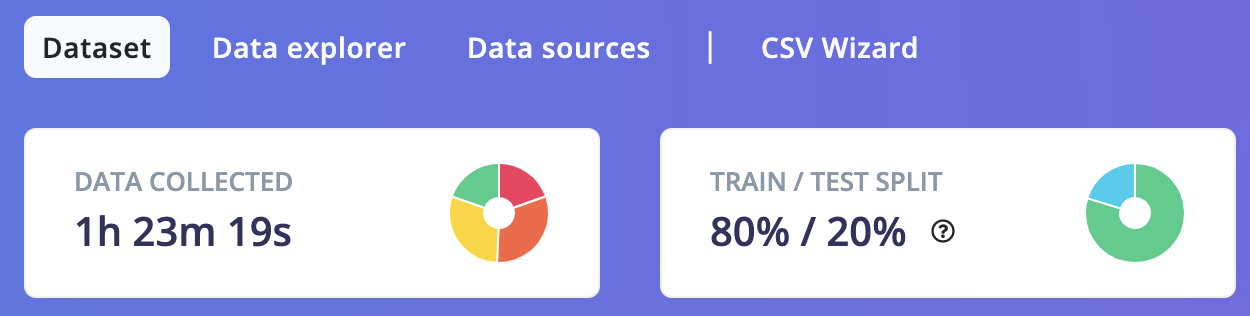
\includegraphics[scale=0.6]{machineLearning/data.png}
    \caption{Once the data is uploaded this figure shows what your project should look like.}
    \label{fig:edgeimpulsedata}
  \end{figure} 

  \item Click on Impulse design
  \item Leave it on Time series data, window of 1000 ms, window increase of 500 ms.
  \item Change the Frequency to 20000 Hz and leave Zero-pad checked
  \item Choose MFCC as the audio features
  \item Classification should have a small number of Output features 
          (4 in my example for no, noise, unknown, yes)
  \item Click Save Impulse
  \item Click on MFCC
  \item Click on Save parameters
  \item Click on the Generate features tab
  \item Then click on the Generate features button. This will take awhile
  \item Once that finishes (green complete in console), click on your model 
          (name under MFCC)
  \item Change the number of training cycles to 50
  \item Change the Learning rate to 0.005
  \item Change the target (upper right) to Raspberry Pi RP2040 (Cortex-M0+ 133MHz)
  \item Click Start training. This will also take awhile.
  \item Once that completes, click on Deployment on the left 
  \item Search deployment options for Arduino library
  \item Click Build
  \item After it finishes it should download a zip file and show some directions
  \item Follow the directions to install the library and open the RP2040 Microphone example 
  \item Try running the example and see if the Serial output shows the word you say as the 
          most likely thing heard. Note that it only listens every few seconds. Watch the 
          serial port output for when it's recording.
\end{enumerate}

\subsection{Using the Recognition}
The library example as written does not output which class is the most likely candidate.
Improve the \lstinline|print_inference_result| function to detect which class has the 
highest likelihood and have it print out that class name and its probability.

Once you have that capability, check to see if the class is one of the spoken words (yes or no vs 
noise or unknown in my example). If it is, play a tone. 

You should also be able to make it drive quite easily as a reaction to your spoken word. To make 
the NeoPixels work, you will need to try a different library. I suspect the screen will not work, but
have not tried it yet.

% need to insert images

% \section{Laboratory}
% \subsection{Download Examples}
% There is a zip file on Canvas named LSM6DSOX\_Examples.zip. Download and extract the zip 
% file. Move the resulting folder into your sketch directory (usually named arduino or Arduino 
% inside your Documents folder). Now try opening one of the examples from within the Arduino IDE.
% If you can find it in your File $\rightarrow$ Sketchbook menu, you have put them in the right
% place.

% \subsection{Install Library}
% Install the STM32duino\_LSM6DSOX library in the Arduino IDE since these examples rely on 
% it for the interface to the IMU.

% \subsection{Running Examples}
% Run each of the following examples noting that the outputs will all be via the serial port:

% \subsubsection{6D Orientation}
% Open the example named LSM6DSOX\_6DOrientation. Compile and upload it to the board. When it
% runs, it should output a drawing indicating the orientation as you rotate the board.

% \subsubsection{Free Fall Detection}
% Don't drop or throw the board! Open the example named LSM6DSOX\_FreeFallDetection. Compile 
% and upload it to your board. When it is running, raise and lower the board while holding it 
% and it should send an output when it thinks it is in free fall. 

% \subsubsection{Pedometer}
% Open the example named LSM6DSOX\_Pedometer. Compile and upload it to the board. Once it is 
% running it should print out the number of steps periodically. Shake the board up and down 
% to imitate walking and it should increment the counter.

% \subsubsection{Tap Detection}
% Open the example named LSM6DSOX\_TapDetect. Compile and upload it to the board. Once it is 
% running try tapping the side of the board/module (not front, back, or top). The serial should 
% output single tap and double tap as it thinks it is tapped.

% \subsubsection{Tilt Detection}
% Open the example named LSM6DSOX\_TiltDetection. Compile and upload it to the board. Once it is 
% running try tilting the board after letting it sit in one orientation for a bit. It should 
% trigger a serial output when you move the board.

% \subsubsection{Wake Up Detection}
% Open the example named LSM6DSOX\_WakeUpDetection. Compile and upload it to the board. Once it is 
% running try moving the board after letting it sit still for a bit. It should trigger a serial 
% output when you move the board.

% \subsubsection{Machine Learning Example}
% Open the example named LSM6DSOX\_MLC. Compile and upload it to the board. Once it is 
% running try moving the board to simulate walking, running, biking, driving, unknown, and 
% staying stationary. Walking and jogging are the easiest to get with vertical motion (Z-axis). 
% Biking seems to be lateral motion (X- or Y-axis). I have seen driving once but don't remember 
% how I got it. I have never seen unknown.

% \subsection{Using the Examples}
% Take one or more of the examples and do something with them. It could be as simple as 
% adding sound or screen output to the example(s) or something more.

% \medskip

% \noindent Have fun!

\section{Turn In}
Turn in the following:
\begin{enumerate}
    \item Have either the TA or the instructor sign-off on your lab
    \item A PDF of your sketch.
    \item .ino versions of your sketch.
    \item Fill out the end of lab quiz prior to leaving. Note that it includes asking you 
            for the output of the \lstinline$getIDs$ sketch. 
\end{enumerate}

\section{Resources}\label{sec:machinelearningresources}
\begin{enumerate}
    \item \href{https://pietropoluzzi.it/blog/ml/edge-impulse/voice-recognition/}{Voice recognition tutorial}
    \item \href{https://docs.edgeimpulse.com/docs/pre-built-datasets/keyword-spotting}{Yes, no, unkown, noise dataset}
    \item \href{https://blog.research.google/2017/08/launching-speech-commands-dataset.html}{Google keywords dataset}
    \item \href{https://github.com/stm32duino/LSM6DSOX/blob/main/src/LSM6DSOXSensor.h}{LSM6DSOX Library Header}
    \item \href{https://www.st.com/resource/en/datasheet/lsm6dsox.pdf}{LSM6DSOX Datasheet}
    \item PCB Schematic and Layout - see 
            \href{https://github.com/semcneil/Fundamentals-of-Microcontrollers-Manual}{class manual} 
            in the Arduino Startup $\rightarrow$ Schematics and PCB section
\end{enumerate}


    \chapter{Controls}
\chaplabel{controls}

\section{Purpose}
The goal of this lab is to play with PID control to get a feel for how it 
works on a real system.

\section{Laboratory}
\subsection{Getting started}
Example code is posted on Canvas as \lstinline@pid_dist_v0.5.ino@. Download and 
try running it. After pressing the right button it should try to maintain a 
distance from an object in front of the robot. The NeoPixels will be red when it 
is in PID mode, and green when it is in HALT mode. Turning the potentiometer
changes the target distance. In order to have the serial port work at the same 
time as the motors run do the following:
\begin{enumerate}
    \item Make sure both motor jumpers are set to BAT 
    \item Plug in the serial port 
    \item Turn on the battery switch.
\end{enumerate}

Make sure this code works as expected. 

\subsection{Proportional Control}
Set the gain for the integral (KI) and derivative (KD) terms to zero. 
Try different values for the proportional control. Can you turn proportional 
control into bang-bang control? How well does it work?

\subsection{Integral Control}
Set the gain for proportional (KP) and derivative (KD) control to zero. 
Try different values for integral control. How well does it run? Can you see 
the windup? What happens for large values of KI? What happens for small values of 
KI?

\subsection{Derivative Control}
Set the gain for proportional (KP) and integral (KI) control to zero.
Try different values for KD. What happens with large values? How about 
for small values?

\subsection{PID Calibration}
Based on the tests you have done so far. Try to find gain values for the 
full PID controller that work better than the defaults in the original file.
How can you tell if your gains are better than the original ones?

\subsection{IMU PID Control}
You have been supplied with a ruler to use as a ramp. Copy the PID file to 
a new one with IMU in the title. Change it to try to level itself by 
backing up the ramp. You will need to use your code for measuring angles 
from a previous lab.

Some other changes that need to be made:
\begin{enumerate}
    \item The distance PID controller is based on \lstinline@int@ values.
            The angle is a float, so the PID function and values need to be 
            updated accordingly.
    \item The error also needs to be changed to a float.
    \item Depending on the angle, the robot may not be able to get onto the
            ramp so you may need to start it on the ramp. Tip the ramp up
            and down to provide perturbances to the system.
    \item The axes that the code measures around need to be changed to 
            measure the front-to-back angle rather than the side-to-side 
            angle.
\end{enumerate}

Be sure to turn off the battery switch prior to putting the robot away.

\section{Turn In}
Turn in the following:
\begin{enumerate}
    \item Have either the TA or the instructor sign-off on your lab
    \item A short writeup with the answers to the questions in the distance PID section.
            One per group is fine.
    \item A PDF of your sketch.
    \item .ino versions of your sketch.
    \item Fill out the end of lab quiz prior to leaving. Note that it includes asking you 
            for the output of the \lstinline$getIDs$ sketch. 
\end{enumerate}

\section{Resources}\label{sec:controlsresources}
\begin{enumerate}
    \item \href{https://github.com/stm32duino/LSM6DSOX/blob/main/src/LSM6DSOXSensor.h}{LSM6DSOX Library Header}
    \item \href{https://www.st.com/resource/en/datasheet/lsm6dsox.pdf}{LSM6DSOX Datasheet}
    \item PCB Schematic and Layout - see 
            \href{https://github.com/semcneil/Fundamentals-of-Microcontrollers-Manual}{class manual} 
            in the Arduino Startup $\rightarrow$ Schematics and PCB section
\end{enumerate}


    \chapter{Wireless}
\chaplabel{wireless}

\section{Purpose}
The goal of this lab is to play with WiFi, Bluetooth, and time. Some of the example
sketches are in a .zip file on Canvas. Download the zip file and unzip it into the 
Arduino directory (typically Documents/Arduino). You should see directories with 
your other sketches inside the Arduino folder.

\section{Laboratory}
\subsection{Preparation}
Before you start this lab, be sure you have updated the following:
\begin{enumerate}
    \item WiFiNINA module firmware
    \item The main libraries used for this lab 
    \begin{enumerate}
        \item WiFiNINA
        \item ArduinoBLE
        \item stm32duino's ST25DV library
    \end{enumerate}
\end{enumerate}

\subsection{WiFi startup}
Follow the WiFiNINA No Encryption example to connect your board to the network. Be 
sure to change the \lstinline|SECRET_SSID| to have \lstinline|EagleNet| between the 
double quotes the \lstinline|arduino_secrets.h| file.

\subsection{NFC}
The ST25DV library is the one in the Arduino Library Manager written by stm32duino.
The library may show as INCOMPATIBLE even though it works fine. Make sure the 
example (NFC\_Demo.ino) from Canvas works as it is supposed to. It should cycle 
different things (website, call, text, etc.) each time you press right the button. Put 
the top of your phone near the coil that says NFC on the bottom left of the robot.

Change the example to show one of your email addresses and the IP address of your 
Nano RP2040 Connect. Demonstrate this to your instructor/TA.

In your code, after WiFi has connected, convert the IPAddress to a \lstinline@String@ 
with the following:\\
\lstinline@IPAddress ip = WiFi.localIP();@\\
\lstinline@String ipString = String(ip[0]) + "." + ip[1] + "." + ip[2] + "." + ip[3];@\\
Now that you have the IP address as a String, you can update \lstinline|NFC_messages| to 
have the IP address String in the correct position. Also update \lstinline|NFC_protocols| 
to use http NOT https. Note that you have to update an element of the \lstinline|NFC_messages| 
array and it has to be done AFTER the WiFi has been setup. This cannot be done where the array is 
initialized before the \lstinline|setup()| function. 


\subsection{UDP Between Boards}
Working with another group, run the examples \lstinline@WiFiUdpSend@ and 
\lstinline@WiFiUdpReceiveSend@ from the Wifi.zip file, one on each of 2 boards. 
Be sure to update \lstinline@remoteIp@ in the 
\lstinline@WiFiUdpSend@ sketch to be the IP address of the other board. Once 
running, the right button on the \lstinline@@ board should turn the LED on 
the other board on and off.

Modify this to do something else (buzzer, NeoPixels, motor, etc.). Demo for the 
instructor/TA.

\subsection{Bluetooth Low Energy}
Be sure to generate your own UUIDs for your particular project. If you use
the UUIDs from the examples, you will not be able to tell if you are connecting
to your board or someone else's who is using the same UUIDs. Use the 
\href{https://www.uuidgenerator.net/}{UUID Generator} to create random UUIDs.
Use UUIDs in the form returned by the website. If you create custom ones with 
a different format, the Bluetooth examples fail.
Be sure to set the device (\lstinline@BLE.setDeviceName@) and local names 
(\lstinline@BLE.setLocalName@) on all boards to something unique to 
your group so that you can find it when scanning.

You will need a Bluetooth app for your phone. Some app names to look for are BlueFruit Connect,
LightBlue, and nRF Connect.

\subsubsection{Phone to Robot Interface}
Use the example code (\lstinline@BLE_ButtonLED@) (being sure to change UUIDs, device name, and local name)
to turn an LED on and off on the robot from your phone. Change the code to 
do something else (buzzer, NeoPixel, motor (carefully), servo) when you change 
the value via the Bluetooth interface. Also, show the button on the board changing
the value read on your phone using the Notify property.

\subsubsection{Inter-Robot Interface}
For this part of the lab you will need to work with another group. Using the example 
of a peripheral (\lstinline@BLE-ButtonLED.ino@) and central (\lstinline@BLE-LED-Central.ino@)
, use one robot to control something on the other robot. Note that you need a different UUID
for each of the peripheral, LED, and Button characteristics but the UUIDs have the be the 
same between the two sketches. Also, the LocalName needs to agree between the sketches.

% This took difficult library installs and seemed to waste time. 
% update it with instructions about what libraries to install
% \subsection{Clock}
% Using the \lstinline@sd-time-logger.ino@ example for setting the 
% RTC for the SD card, write a program that gets the current time, 
% then displays the time in the format HH:MM:SS and the date 
% (on a different line) in the format YYYY-MM-DD on the display 
% that updates each second. Install the \lstinline@RP2040_RTC@ 
% library with NONE of the other dependencies. 

\subsection{AJAX}
There are 3 files on Canvas:
\begin{enumerate}
    \item AJAX-Robot.ino 
    \item arduino\_secrets.h
    \item index.h 
\end{enumerate}
Open the .ino file and then put the other files in the same directory. Make sure
to add them to the sketch (Sketch$\rightarrow$Add File) so that they show up as separate 
tabs. Upload the file to the robot. Once it has uploaded and the LEDs are green,
put your phone next to the NFC and go to the URL listed (you must be on the 
EagleNet WiFi for it to load). Once you are on the site you can control the 
builtin LED, the servo position, and the NeoPixel color as well as read the 
distance measurement.

\section{Shutdown}
Be sure to turn off the battery switch prior to putting the robot away.

\section{Turn In}
Turn in the following:
\begin{enumerate}
    \item Have either the TA or the instructor sign-off on your lab
    \item A PDF of your NFC sketch.
    \item .ino versions of your NFC sketch.
    \item Fill out the end of lab quiz prior to leaving. Note that it includes asking you 
            for the output of the \lstinline$getIDs$ sketch. 
\end{enumerate}

\section{Resources}\label{sec:wirelessresources}
\begin{enumerate}
    \item \href{https://www.uuidgenerator.net/}{UUID Generator} 
    \item PCB Schematic and Layout - see 
            \href{https://github.com/semcneil/Fundamentals-of-Microcontrollers-Manual}{class manual} 
            in the Arduino Startup $\rightarrow$ Schematics and PCB section
\end{enumerate}
This explains some of the code you are using.
\subsubsection{Peripheral Setup}
\begin{enumerate}
    \item Include Arduino's BLE library \\
        \lstinline@#include <ArduinoBLE.h>@ 
    \item Create a BLEService. This is container for characteristics. You can
            have multiple services and characteristics per service.\\
        \lstinline@BLEService ledService(String UUID);@
    \item Create a variable for each characteristic. Characteristics have properties. 
            The most used properties are:
        \begin{enumerate}
            \item BLERead - This allows a connected device to read the value of this variable
            \item BLEWrite - This allows a connected device to change the value of the variable
            \item BLENotify -  This allows a connected device to be notified if the value changes
        \end{enumerate}
        \lstinline@BLEByteCharacteristic LEDCharacteristic(String UUID, BLERead | BLEWrite);@ \\
        \lstinline@BLEByteCharacteristic buttonCharacteristic(String UUID, BLERead | BLENotify);@
    \item The next setup is done in the \lstinline@setup()@ function
    \item Start the BLE module \\
        \lstinline@BLE.begin()@ 
    \item Set the device name. This is the externally advertised name \\
        \lstinline@BLE.setDeviceName("BUTTON_LED");@ 
    \item Set the local name. This can be checked by a device once connected \\
        \lstinline@BLE.setLocalName("BUTTON_LED_MCNEILL");@ 
    \item Set the service as advertised \\
        \lstinline@BLE.setAdvertisedService(ledService);@
    \item Add the characteristics to the service \\
        \lstinline@ledService.addCharacteristic(LEDCharacteristic);@
    \item Add the service to the BLE object \\
        \lstinline@BLE.addService(ledService);@
    \item Set initial values for each characteristic \\
        \lstinline@LEDCharacteristic.writeValue(0);@
    \item Finish by starting your BLE advertising its existence \\
        \lstinline@BLE.advertise();@
    \item In the \lstinline@loop()@ my preferred method is to create central device
            and check to see if a device has connected. Once it has, update the 
            values of the output characteristics and check if the writeable 
            characteristics have been written to.
\end{enumerate}
\subsubsection{Central Setup}
\begin{enumerate}
    \item Scan for a device, typically by service UUID. \\
        \lstinline@BLE.scanForUuid(BLE_UUID_PERIPHERAL);@ 
    \item Create a peripheral object \\
        \lstinline@BLEDevice peripheral = BLE.available();@ 
    \item If the peripheral has been discovered, check its local name  \\
        \lstinline@if (peripheral.localName() != "BUTTON_LED")@ 
    \item Stop scanning \\
        \lstinline@BLE.stopScan();@ 
    \item Connect to the peripheral \\
        \lstinline@peripheral.connect()@ 
    \item Read the peripheral's attributes \\
        \lstinline@peripheral.discoverAttributes()@ 
    \item Retrieve each characteristic and check to make sure each has the 
            attributes (Read/Write/Notify) expected
        \begin{lstlisting}
if (!buttonCharacteristic) {
    Serial.println("Peripheral does not have button characteristic!");
    peripheral.disconnect();
    return;
} else if (!buttonCharacteristic.canRead()) {
    Serial.println("Peripheral does not have a readable button characteristic!");
    peripheral.disconnect();
    return;
} else if (!buttonCharacteristic.canSubscribe()) {
    Serial.println("Peripheral does not allow button subscriptions (notify)");
} else if(!buttonCharacteristic.subscribe()) {
    Serial.println("Subscription failed!");
} else {
    Serial.println("Connected to button characteristic");
}
        \end{lstlisting}
    \item Read/write the peripheral's characteristics as desired
        \begin{lstlisting}
if(buttonCharacteristic && buttonCharacteristic.canRead() && buttonCharacteristic.valueUpdated()) {
    byte peripheralButtonState;
    buttonCharacteristic.readValue(peripheralButtonState);
    if(!peripheralButtonState) {
        digitalWrite(ledPin, HIGH);
    } else {
        digitalWrite(ledPin, LOW);
    }
}          
        \end{lstlisting}
\end{enumerate}



\end{document}